\documentclass[twoside]{book}

% Packages required by doxygen
\usepackage{fixltx2e}
\usepackage{calc}
\usepackage{doxygen}
\usepackage[export]{adjustbox} % also loads graphicx
\usepackage{graphicx}
\usepackage[utf8]{inputenc}
\usepackage{makeidx}
\usepackage{multicol}
\usepackage{multirow}
\PassOptionsToPackage{warn}{textcomp}
\usepackage{textcomp}
\usepackage[nointegrals]{wasysym}
\usepackage[table]{xcolor}

% NLS support packages
\usepackage{polski}
\usepackage[T1]{fontenc}

% Font selection
\usepackage[T1]{fontenc}
\usepackage[scaled=.90]{helvet}
\usepackage{courier}
\usepackage{amssymb}
\usepackage{sectsty}
\renewcommand{\familydefault}{\sfdefault}
\allsectionsfont{%
  \fontseries{bc}\selectfont%
  \color{darkgray}%
}
\renewcommand{\DoxyLabelFont}{%
  \fontseries{bc}\selectfont%
  \color{darkgray}%
}
\newcommand{\+}{\discretionary{\mbox{\scriptsize$\hookleftarrow$}}{}{}}

% Page & text layout
\usepackage{geometry}
\geometry{%
  a4paper,%
  top=2.5cm,%
  bottom=2.5cm,%
  left=2.5cm,%
  right=2.5cm%
}
\tolerance=750
\hfuzz=15pt
\hbadness=750
\setlength{\emergencystretch}{15pt}
\setlength{\parindent}{0cm}
\setlength{\parskip}{3ex plus 2ex minus 2ex}
\makeatletter
\renewcommand{\paragraph}{%
  \@startsection{paragraph}{4}{0ex}{-1.0ex}{1.0ex}{%
    \normalfont\normalsize\bfseries\SS@parafont%
  }%
}
\renewcommand{\subparagraph}{%
  \@startsection{subparagraph}{5}{0ex}{-1.0ex}{1.0ex}{%
    \normalfont\normalsize\bfseries\SS@subparafont%
  }%
}
\makeatother

% Headers & footers
\usepackage{fancyhdr}
\pagestyle{fancyplain}
\fancyhead[LE]{\fancyplain{}{\bfseries\thepage}}
\fancyhead[CE]{\fancyplain{}{}}
\fancyhead[RE]{\fancyplain{}{\bfseries\leftmark}}
\fancyhead[LO]{\fancyplain{}{\bfseries\rightmark}}
\fancyhead[CO]{\fancyplain{}{}}
\fancyhead[RO]{\fancyplain{}{\bfseries\thepage}}
\fancyfoot[LE]{\fancyplain{}{}}
\fancyfoot[CE]{\fancyplain{}{}}
\fancyfoot[RE]{\fancyplain{}{\bfseries\scriptsize Wygenerowano przez Doxygen }}
\fancyfoot[LO]{\fancyplain{}{\bfseries\scriptsize Wygenerowano przez Doxygen }}
\fancyfoot[CO]{\fancyplain{}{}}
\fancyfoot[RO]{\fancyplain{}{}}
\renewcommand{\footrulewidth}{0.4pt}
\renewcommand{\chaptermark}[1]{%
  \markboth{#1}{}%
}
\renewcommand{\sectionmark}[1]{%
  \markright{\thesection\ #1}%
}

% Indices & bibliography
\usepackage{natbib}
\usepackage[titles]{tocloft}
\setcounter{tocdepth}{3}
\setcounter{secnumdepth}{5}
\makeindex

% Hyperlinks (required, but should be loaded last)
\usepackage{ifpdf}
\ifpdf
  \usepackage[pdftex,pagebackref=true]{hyperref}
\else
  \usepackage[ps2pdf,pagebackref=true]{hyperref}
\fi
\hypersetup{%
  colorlinks=true,%
  linkcolor=blue,%
  citecolor=blue,%
  unicode%
}

% Custom commands
\newcommand{\clearemptydoublepage}{%
  \newpage{\pagestyle{empty}\cleardoublepage}%
}

\usepackage{caption}
\captionsetup{labelsep=space,justification=centering,font={bf},singlelinecheck=off,skip=4pt,position=top}

%===== C O N T E N T S =====

\begin{document}

% Titlepage & ToC
\hypersetup{pageanchor=false,
             bookmarksnumbered=true,
             pdfencoding=unicode
            }
\pagenumbering{alph}
\begin{titlepage}
\vspace*{7cm}
\begin{center}%
{\Large Drzewo B\+ST }\\
\vspace*{1cm}
{\large Wygenerowano przez Doxygen 1.8.14}\\
\end{center}
\end{titlepage}
\clearemptydoublepage
\pagenumbering{roman}
\tableofcontents
\clearemptydoublepage
\pagenumbering{arabic}
\hypersetup{pageanchor=true}

%--- Begin generated contents ---
\chapter{Indeks hierarchiczny}
\section{Hierarchia klas}
Ta lista dziedziczenia posortowana jest z grubsza, choć nie całkowicie, alfabetycznie\+:\begin{DoxyCompactList}
\item \contentsline{section}{B\+ST}{\pageref{class_b_s_t}}{}
\item \contentsline{section}{tekstura}{\pageref{classtekstura}}{}
\item \contentsline{section}{tekstury}{\pageref{classtekstury}}{}
\item \contentsline{section}{wezel}{\pageref{classwezel}}{}
\item wx\+Dialog\begin{DoxyCompactList}
\item \contentsline{section}{New\+Dialog}{\pageref{class_new_dialog}}{}
\end{DoxyCompactList}
\end{DoxyCompactList}

\chapter{Indeks klas}
\section{Lista klas}
Tutaj znajdują się klasy, struktury, unie i interfejsy wraz z ich krótkimi opisami\+:\begin{DoxyCompactList}
\item\contentsline{section}{\mbox{\hyperlink{class_b_s_t}{B\+ST}} \\*Definicja klasy \mbox{\hyperlink{class_b_s_t}{B\+ST}} }{\pageref{class_b_s_t}}{}
\item\contentsline{section}{\mbox{\hyperlink{class_new_dialog}{New\+Dialog}} }{\pageref{class_new_dialog}}{}
\item\contentsline{section}{\mbox{\hyperlink{classtekstura}{tekstura}} \\*Definicja klasy tekstura }{\pageref{classtekstura}}{}
\item\contentsline{section}{\mbox{\hyperlink{classtekstury}{tekstury}} \\*Definicja klasy tekstury }{\pageref{classtekstury}}{}
\item\contentsline{section}{\mbox{\hyperlink{classwezel}{wezel}} \\*Definicja klasy wezel }{\pageref{classwezel}}{}
\end{DoxyCompactList}

\chapter{Indeks plików}
\section{Lista plików}
Tutaj znajduje się lista wszystkich plików z ich krótkimi opisami\+:\begin{DoxyCompactList}
\item\contentsline{section}{C\+:/cpp/drzewo\+\_\+bst/\mbox{\hyperlink{bst_8cpp}{bst.\+cpp}} \\*Plik zawierający implementację metod klasy \mbox{\hyperlink{class_b_s_t}{B\+ST}} }{\pageref{bst_8cpp}}{}
\item\contentsline{section}{C\+:/cpp/drzewo\+\_\+bst/\mbox{\hyperlink{bst_8h}{bst.\+h}} \\*Plik zawierający definicje klas dla drzewa \mbox{\hyperlink{class_b_s_t}{B\+ST}} }{\pageref{bst_8h}}{}
\item\contentsline{section}{C\+:/cpp/drzewo\+\_\+bst/\mbox{\hyperlink{funkcje_8cpp}{funkcje.\+cpp}} \\*Plik zawierający implementacje funkcji ogólnego przeznaczenia }{\pageref{funkcje_8cpp}}{}
\item\contentsline{section}{C\+:/cpp/drzewo\+\_\+bst/\mbox{\hyperlink{funkcje_8h}{funkcje.\+h}} \\*Plik zawierający nagłówki funkcji ogólnego przeznaczenia }{\pageref{funkcje_8h}}{}
\item\contentsline{section}{C\+:/cpp/drzewo\+\_\+bst/\mbox{\hyperlink{main_8cpp}{main.\+cpp}} \\*Plik zawierający funkcję główną programu }{\pageref{main_8cpp}}{}
\item\contentsline{section}{C\+:/cpp/drzewo\+\_\+bst/\mbox{\hyperlink{_new_dialog_8cpp}{New\+Dialog.\+cpp}} }{\pageref{_new_dialog_8cpp}}{}
\item\contentsline{section}{C\+:/cpp/drzewo\+\_\+bst/\mbox{\hyperlink{_new_dialog_8h}{New\+Dialog.\+h}} }{\pageref{_new_dialog_8h}}{}
\item\contentsline{section}{C\+:/cpp/drzewo\+\_\+bst/\mbox{\hyperlink{resource_8h}{resource.\+h}} }{\pageref{resource_8h}}{}
\item\contentsline{section}{C\+:/cpp/drzewo\+\_\+bst/\mbox{\hyperlink{tekstury_8cpp}{tekstury.\+cpp}} \\*Plik zawierający implementację metod obsługujących tekstury Open\+GL }{\pageref{tekstury_8cpp}}{}
\item\contentsline{section}{C\+:/cpp/drzewo\+\_\+bst/\mbox{\hyperlink{tekstury_8h}{tekstury.\+h}} \\*Plik zawierający definicje klas odpowiedzialnych za tekstury Open\+GL wykorzystywane w programie }{\pageref{tekstury_8h}}{}
\end{DoxyCompactList}

\chapter{Dokumentacja klas}
\hypertarget{class_b_s_t}{}\section{Dokumentacja klasy B\+ST}
\label{class_b_s_t}\index{B\+ST@{B\+ST}}


Definicja klasy \mbox{\hyperlink{class_b_s_t}{B\+ST}}.  




{\ttfamily \#include $<$bst.\+h$>$}

\subsection*{Metody publiczne}
\begin{DoxyCompactItemize}
\item 
\mbox{\hyperlink{class_b_s_t_abc17123a0367c3b8ad0382eeb3ad3178}{B\+ST}} ()
\item 
void \mbox{\hyperlink{class_b_s_t_ae5f20b665705c82452690ba682f867a6}{generuj\+\_\+nowe}} (int ile, int zakres, int uporzadkowanie)
\item 
void \mbox{\hyperlink{class_b_s_t_a14df9d739a34fd8c391c07df9e5ca1d3}{dodaj}} (int wartosc)
\item 
\mbox{\hyperlink{classwezel}{wezel}} $\ast$ \mbox{\hyperlink{class_b_s_t_a1b0748887eae594e90cfe2494baa29ea}{wyszukaj}} (int klucz)
\item 
void \mbox{\hyperlink{class_b_s_t_acd478acd615c38053ca2e28e217c43fe}{wyczysc\+\_\+wyszukiwanie}} (\mbox{\hyperlink{classwezel}{wezel}} $\ast$W)
\item 
\mbox{\hyperlink{classwezel}{wezel}} $\ast$ \mbox{\hyperlink{class_b_s_t_a67b2888aec856d1e00e569a1feabf905}{usun}} (\mbox{\hyperlink{classwezel}{wezel}} $\ast$x)
\item 
void \mbox{\hyperlink{class_b_s_t_a538330cbdb455f7e676db5ee9ef29f54}{wyswietl}} (int x, int y, int rozpietosc, \mbox{\hyperlink{classwezel}{wezel}} $\ast$W, int kolor, \mbox{\hyperlink{classtekstury}{tekstury}} $\ast$\mbox{\hyperlink{main_8cpp_ab6e212a94c16ea306129c2e8e004bd6f}{T}})
\item 
void \mbox{\hyperlink{class_b_s_t_a7605bbad3398366c380300c97eed9ace}{wyswietl\+\_\+drzewo}} (\mbox{\hyperlink{classtekstury}{tekstury}} $\ast$\mbox{\hyperlink{main_8cpp_ab6e212a94c16ea306129c2e8e004bd6f}{T}})
\end{DoxyCompactItemize}
\subsection*{Atrybuty publiczne}
\begin{DoxyCompactItemize}
\item 
\mbox{\hyperlink{classwezel}{wezel}} $\ast$ \mbox{\hyperlink{class_b_s_t_a8b2f27f4b58aceda99b397e3f5447e6a}{korzen}}
\item 
int \mbox{\hyperlink{class_b_s_t_a7c4c3ea4245b2eb6e0c87720743c03b4}{liczba\+\_\+porownan}}
\item 
int \mbox{\hyperlink{class_b_s_t_abd1f7811c4077eecacb5a4ab2013ef53}{liczba\+\_\+przebiegow\+\_\+petli}}
\item 
int \mbox{\hyperlink{class_b_s_t_a8d4e71cbb02976259d9893169ea2b6ac}{liczba\+\_\+przypisan}}
\end{DoxyCompactItemize}


\subsection{Opis szczegółowy}
Definicja klasy \mbox{\hyperlink{class_b_s_t}{B\+ST}}. 

Klasa \mbox{\hyperlink{class_b_s_t}{B\+ST}} przechowuje wskaźnik do drzewa \mbox{\hyperlink{class_b_s_t}{B\+ST}} oraz zawiera metody zarządzające drzewem. 

\subsection{Dokumentacja konstruktora i destruktora}
\mbox{\Hypertarget{class_b_s_t_abc17123a0367c3b8ad0382eeb3ad3178}\label{class_b_s_t_abc17123a0367c3b8ad0382eeb3ad3178}} 
\index{B\+ST@{B\+ST}!B\+ST@{B\+ST}}
\index{B\+ST@{B\+ST}!B\+ST@{B\+ST}}
\subsubsection{\texorpdfstring{B\+S\+T()}{BST()}}
{\footnotesize\ttfamily B\+S\+T\+::\+B\+ST (\begin{DoxyParamCaption}{ }\end{DoxyParamCaption})}

konstruktor klasy \mbox{\hyperlink{class_b_s_t}{B\+ST}} 

\subsection{Dokumentacja funkcji składowych}
\mbox{\Hypertarget{class_b_s_t_a14df9d739a34fd8c391c07df9e5ca1d3}\label{class_b_s_t_a14df9d739a34fd8c391c07df9e5ca1d3}} 
\index{B\+ST@{B\+ST}!dodaj@{dodaj}}
\index{dodaj@{dodaj}!B\+ST@{B\+ST}}
\subsubsection{\texorpdfstring{dodaj()}{dodaj()}}
{\footnotesize\ttfamily void B\+S\+T\+::dodaj (\begin{DoxyParamCaption}\item[{int}]{wartosc }\end{DoxyParamCaption})}

metoda dodająca nowy węzeł do drzewa 
\begin{DoxyParams}{Parametry}
{\em wartosc} & określa wartość, która będzie wstawiona do węzła \\
\hline
\end{DoxyParams}
\mbox{\Hypertarget{class_b_s_t_ae5f20b665705c82452690ba682f867a6}\label{class_b_s_t_ae5f20b665705c82452690ba682f867a6}} 
\index{B\+ST@{B\+ST}!generuj\+\_\+nowe@{generuj\+\_\+nowe}}
\index{generuj\+\_\+nowe@{generuj\+\_\+nowe}!B\+ST@{B\+ST}}
\subsubsection{\texorpdfstring{generuj\+\_\+nowe()}{generuj\_nowe()}}
{\footnotesize\ttfamily void B\+S\+T\+::generuj\+\_\+nowe (\begin{DoxyParamCaption}\item[{int}]{ile,  }\item[{int}]{zakres,  }\item[{int}]{uporzadkowanie }\end{DoxyParamCaption})}

metoda generująca nowe drzewo 
\begin{DoxyParams}{Parametry}
{\em ile} & liczba węzłów \\
\hline
{\em zakres} & zakres generowanych wartości węzła \\
\hline
{\em uporzadkowanie} & rodzaj uporządkowania \\
\hline
\end{DoxyParams}
\mbox{\Hypertarget{class_b_s_t_a67b2888aec856d1e00e569a1feabf905}\label{class_b_s_t_a67b2888aec856d1e00e569a1feabf905}} 
\index{B\+ST@{B\+ST}!usun@{usun}}
\index{usun@{usun}!B\+ST@{B\+ST}}
\subsubsection{\texorpdfstring{usun()}{usun()}}
{\footnotesize\ttfamily \mbox{\hyperlink{classwezel}{wezel}} $\ast$ B\+S\+T\+::usun (\begin{DoxyParamCaption}\item[{\mbox{\hyperlink{classwezel}{wezel}} $\ast$}]{x }\end{DoxyParamCaption})}

metoda usuwająca węzeł \mbox{\Hypertarget{class_b_s_t_acd478acd615c38053ca2e28e217c43fe}\label{class_b_s_t_acd478acd615c38053ca2e28e217c43fe}} 
\index{B\+ST@{B\+ST}!wyczysc\+\_\+wyszukiwanie@{wyczysc\+\_\+wyszukiwanie}}
\index{wyczysc\+\_\+wyszukiwanie@{wyczysc\+\_\+wyszukiwanie}!B\+ST@{B\+ST}}
\subsubsection{\texorpdfstring{wyczysc\+\_\+wyszukiwanie()}{wyczysc\_wyszukiwanie()}}
{\footnotesize\ttfamily void B\+S\+T\+::wyczysc\+\_\+wyszukiwanie (\begin{DoxyParamCaption}\item[{\mbox{\hyperlink{classwezel}{wezel}} $\ast$}]{W }\end{DoxyParamCaption})}

metoda czyszcząca węzły kolorowane w trakcie wyszukiwania \mbox{\Hypertarget{class_b_s_t_a538330cbdb455f7e676db5ee9ef29f54}\label{class_b_s_t_a538330cbdb455f7e676db5ee9ef29f54}} 
\index{B\+ST@{B\+ST}!wyswietl@{wyswietl}}
\index{wyswietl@{wyswietl}!B\+ST@{B\+ST}}
\subsubsection{\texorpdfstring{wyswietl()}{wyswietl()}}
{\footnotesize\ttfamily void B\+S\+T\+::wyswietl (\begin{DoxyParamCaption}\item[{int}]{x,  }\item[{int}]{y,  }\item[{int}]{rozpietosc,  }\item[{\mbox{\hyperlink{classwezel}{wezel}} $\ast$}]{W,  }\item[{int}]{kolor,  }\item[{\mbox{\hyperlink{classtekstury}{tekstury}} $\ast$}]{T }\end{DoxyParamCaption})}

metoda wyświetlająca węzeł drzewa 
\begin{DoxyParams}{Parametry}
{\em x} & pozycja x na ekranie \\
\hline
{\em y} & pozycja y na ekranie \\
\hline
{\em rozpietosc} & odległość między węzłami potomnymi \\
\hline
{\em W} & wskaźnik na węzeł \\
\hline
{\em kolor} & kolor węzła (niebieski -\/ korzeń, czerwony -\/ prawy potomek, zielony -\/ lewy potomek) \\
\hline
{\em T} & wskaźnik na obiekt przechowujący tekstury \\
\hline
\end{DoxyParams}
\mbox{\Hypertarget{class_b_s_t_a7605bbad3398366c380300c97eed9ace}\label{class_b_s_t_a7605bbad3398366c380300c97eed9ace}} 
\index{B\+ST@{B\+ST}!wyswietl\+\_\+drzewo@{wyswietl\+\_\+drzewo}}
\index{wyswietl\+\_\+drzewo@{wyswietl\+\_\+drzewo}!B\+ST@{B\+ST}}
\subsubsection{\texorpdfstring{wyswietl\+\_\+drzewo()}{wyswietl\_drzewo()}}
{\footnotesize\ttfamily void B\+S\+T\+::wyswietl\+\_\+drzewo (\begin{DoxyParamCaption}\item[{\mbox{\hyperlink{classtekstury}{tekstury}} $\ast$}]{T }\end{DoxyParamCaption})}

metoda wyświetlająca całe drzewo \mbox{\hyperlink{class_b_s_t}{B\+ST}} 
\begin{DoxyParams}{Parametry}
{\em T} & wskaźnik na obiekt przechowujący tekstury \\
\hline
\end{DoxyParams}
\mbox{\Hypertarget{class_b_s_t_a1b0748887eae594e90cfe2494baa29ea}\label{class_b_s_t_a1b0748887eae594e90cfe2494baa29ea}} 
\index{B\+ST@{B\+ST}!wyszukaj@{wyszukaj}}
\index{wyszukaj@{wyszukaj}!B\+ST@{B\+ST}}
\subsubsection{\texorpdfstring{wyszukaj()}{wyszukaj()}}
{\footnotesize\ttfamily \mbox{\hyperlink{classwezel}{wezel}} $\ast$ B\+S\+T\+::wyszukaj (\begin{DoxyParamCaption}\item[{int}]{klucz }\end{DoxyParamCaption})}

metoda wyszukująca węzła o podanej wartości klucza 

\subsection{Dokumentacja atrybutów składowych}
\mbox{\Hypertarget{class_b_s_t_a8b2f27f4b58aceda99b397e3f5447e6a}\label{class_b_s_t_a8b2f27f4b58aceda99b397e3f5447e6a}} 
\index{B\+ST@{B\+ST}!korzen@{korzen}}
\index{korzen@{korzen}!B\+ST@{B\+ST}}
\subsubsection{\texorpdfstring{korzen}{korzen}}
{\footnotesize\ttfamily \mbox{\hyperlink{classwezel}{wezel}}$\ast$ B\+S\+T\+::korzen}

wskaźnik na korzeń drzewa \mbox{\Hypertarget{class_b_s_t_a7c4c3ea4245b2eb6e0c87720743c03b4}\label{class_b_s_t_a7c4c3ea4245b2eb6e0c87720743c03b4}} 
\index{B\+ST@{B\+ST}!liczba\+\_\+porownan@{liczba\+\_\+porownan}}
\index{liczba\+\_\+porownan@{liczba\+\_\+porownan}!B\+ST@{B\+ST}}
\subsubsection{\texorpdfstring{liczba\+\_\+porownan}{liczba\_porownan}}
{\footnotesize\ttfamily int B\+S\+T\+::liczba\+\_\+porownan}

liczba porównań (statystyczna) \mbox{\Hypertarget{class_b_s_t_abd1f7811c4077eecacb5a4ab2013ef53}\label{class_b_s_t_abd1f7811c4077eecacb5a4ab2013ef53}} 
\index{B\+ST@{B\+ST}!liczba\+\_\+przebiegow\+\_\+petli@{liczba\+\_\+przebiegow\+\_\+petli}}
\index{liczba\+\_\+przebiegow\+\_\+petli@{liczba\+\_\+przebiegow\+\_\+petli}!B\+ST@{B\+ST}}
\subsubsection{\texorpdfstring{liczba\+\_\+przebiegow\+\_\+petli}{liczba\_przebiegow\_petli}}
{\footnotesize\ttfamily int B\+S\+T\+::liczba\+\_\+przebiegow\+\_\+petli}

liczba przebiegów pętli (statystyczna) \mbox{\Hypertarget{class_b_s_t_a8d4e71cbb02976259d9893169ea2b6ac}\label{class_b_s_t_a8d4e71cbb02976259d9893169ea2b6ac}} 
\index{B\+ST@{B\+ST}!liczba\+\_\+przypisan@{liczba\+\_\+przypisan}}
\index{liczba\+\_\+przypisan@{liczba\+\_\+przypisan}!B\+ST@{B\+ST}}
\subsubsection{\texorpdfstring{liczba\+\_\+przypisan}{liczba\_przypisan}}
{\footnotesize\ttfamily int B\+S\+T\+::liczba\+\_\+przypisan}

liczba przypisań (statystyczna) 

Dokumentacja dla tej klasy została wygenerowana z plików\+:\begin{DoxyCompactItemize}
\item 
C\+:/cpp/drzewo\+\_\+bst/\mbox{\hyperlink{bst_8h}{bst.\+h}}\item 
C\+:/cpp/drzewo\+\_\+bst/\mbox{\hyperlink{bst_8cpp}{bst.\+cpp}}\end{DoxyCompactItemize}

\hypertarget{class_new_dialog}{}\section{Dokumentacja klasy New\+Dialog}
\label{class_new_dialog}\index{New\+Dialog@{New\+Dialog}}


{\ttfamily \#include $<$New\+Dialog.\+h$>$}

Diagram dziedziczenia dla New\+Dialog\begin{figure}[H]
\begin{center}
\leavevmode
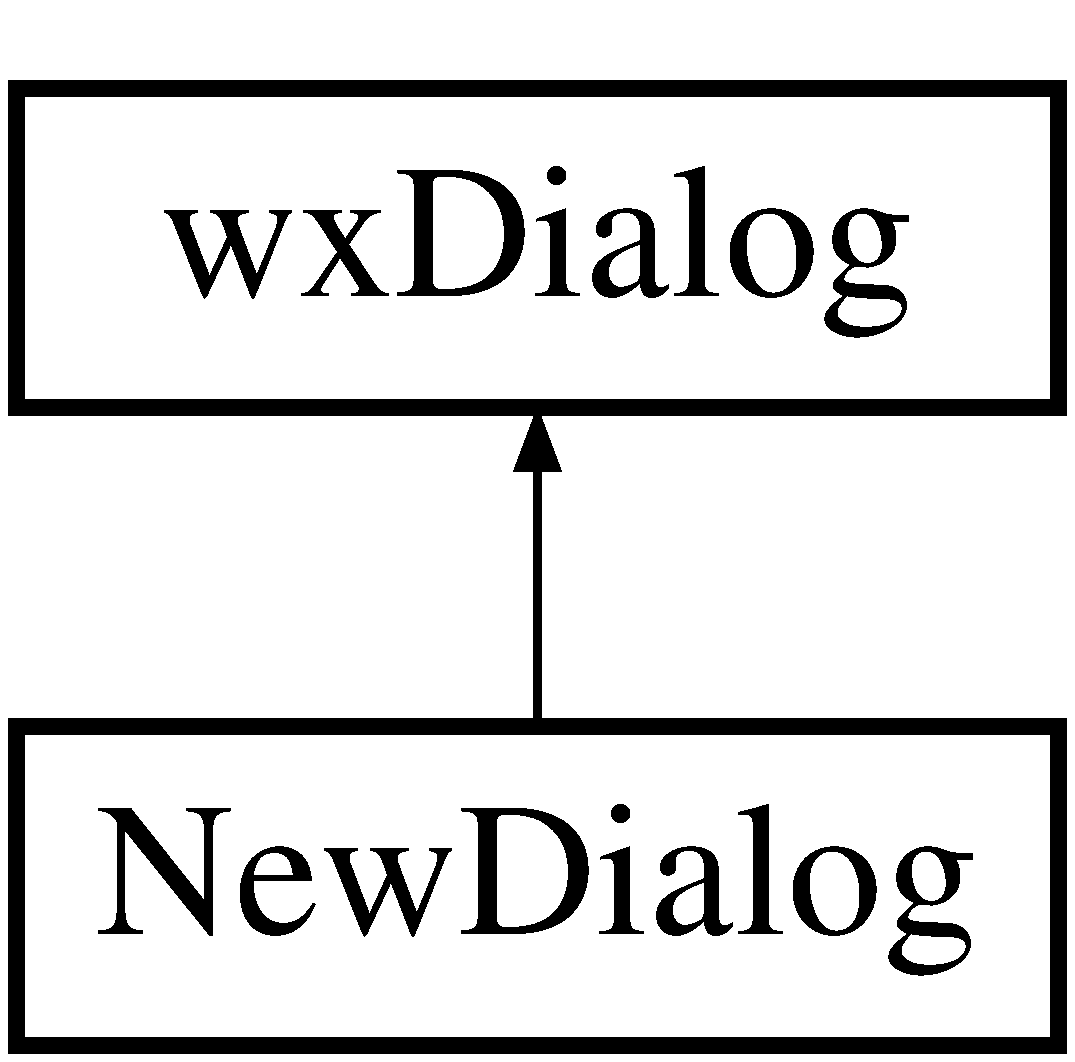
\includegraphics[height=2.000000cm]{class_new_dialog}
\end{center}
\end{figure}
\subsection*{Metody publiczne}
\begin{DoxyCompactItemize}
\item 
\mbox{\hyperlink{class_new_dialog_a6910ade228aac35f03cb8840d12b79f7}{New\+Dialog}} (wx\+Window $\ast$parent, wx\+Window\+ID id=wx\+I\+D\+\_\+\+A\+NY)
\item 
virtual \mbox{\hyperlink{class_new_dialog_a971b50e63d72ee512ccf6df01725afa4}{$\sim$\+New\+Dialog}} ()
\end{DoxyCompactItemize}
\subsection*{Atrybuty publiczne}
\begin{DoxyCompactItemize}
\item 
wx\+Text\+Ctrl $\ast$ \mbox{\hyperlink{class_new_dialog_a49642e1118d27d204d51b3fefa910436}{wartosc}}
\item 
wx\+Button $\ast$ \mbox{\hyperlink{class_new_dialog_ad15bf2122e8f06769d1c05f1bc57ce37}{Przycisk}}
\item 
wx\+Static\+Text $\ast$ \mbox{\hyperlink{class_new_dialog_a55766963c57d72db947c9cddae1dbf61}{Static\+Text1}}
\end{DoxyCompactItemize}
\subsection*{Statyczne atrybuty chronione}
\begin{DoxyCompactItemize}
\item 
static const long \mbox{\hyperlink{class_new_dialog_a7a0d550ea58e2fadee155ac45a46c685}{I\+D\+\_\+\+S\+T\+A\+T\+I\+C\+T\+E\+X\+T1}} = wx\+New\+Id()
\item 
static const long \mbox{\hyperlink{class_new_dialog_a873b13e70226c0c50c58a2a31e7c5e6a}{I\+D\+\_\+\+T\+E\+X\+T\+C\+T\+R\+L1}} = wx\+New\+Id()
\item 
static const long \mbox{\hyperlink{class_new_dialog_a19d3f77775795f2dffa1c779f42e26e6}{I\+D\+\_\+\+B\+U\+T\+T\+O\+N1}} = wx\+New\+Id()
\end{DoxyCompactItemize}


\subsection{Dokumentacja konstruktora i destruktora}
\mbox{\Hypertarget{class_new_dialog_a6910ade228aac35f03cb8840d12b79f7}\label{class_new_dialog_a6910ade228aac35f03cb8840d12b79f7}} 
\index{New\+Dialog@{New\+Dialog}!New\+Dialog@{New\+Dialog}}
\index{New\+Dialog@{New\+Dialog}!New\+Dialog@{New\+Dialog}}
\subsubsection{\texorpdfstring{New\+Dialog()}{NewDialog()}}
{\footnotesize\ttfamily New\+Dialog\+::\+New\+Dialog (\begin{DoxyParamCaption}\item[{wx\+Window $\ast$}]{parent,  }\item[{wx\+Window\+ID}]{id = {\ttfamily wxID\+\_\+ANY} }\end{DoxyParamCaption})}

\mbox{\Hypertarget{class_new_dialog_a971b50e63d72ee512ccf6df01725afa4}\label{class_new_dialog_a971b50e63d72ee512ccf6df01725afa4}} 
\index{New\+Dialog@{New\+Dialog}!````~New\+Dialog@{$\sim$\+New\+Dialog}}
\index{````~New\+Dialog@{$\sim$\+New\+Dialog}!New\+Dialog@{New\+Dialog}}
\subsubsection{\texorpdfstring{$\sim$\+New\+Dialog()}{~NewDialog()}}
{\footnotesize\ttfamily New\+Dialog\+::$\sim$\+New\+Dialog (\begin{DoxyParamCaption}{ }\end{DoxyParamCaption})\hspace{0.3cm}{\ttfamily [virtual]}}



\subsection{Dokumentacja atrybutów składowych}
\mbox{\Hypertarget{class_new_dialog_a19d3f77775795f2dffa1c779f42e26e6}\label{class_new_dialog_a19d3f77775795f2dffa1c779f42e26e6}} 
\index{New\+Dialog@{New\+Dialog}!I\+D\+\_\+\+B\+U\+T\+T\+O\+N1@{I\+D\+\_\+\+B\+U\+T\+T\+O\+N1}}
\index{I\+D\+\_\+\+B\+U\+T\+T\+O\+N1@{I\+D\+\_\+\+B\+U\+T\+T\+O\+N1}!New\+Dialog@{New\+Dialog}}
\subsubsection{\texorpdfstring{I\+D\+\_\+\+B\+U\+T\+T\+O\+N1}{ID\_BUTTON1}}
{\footnotesize\ttfamily const long New\+Dialog\+::\+I\+D\+\_\+\+B\+U\+T\+T\+O\+N1 = wx\+New\+Id()\hspace{0.3cm}{\ttfamily [static]}, {\ttfamily [protected]}}

\mbox{\Hypertarget{class_new_dialog_a7a0d550ea58e2fadee155ac45a46c685}\label{class_new_dialog_a7a0d550ea58e2fadee155ac45a46c685}} 
\index{New\+Dialog@{New\+Dialog}!I\+D\+\_\+\+S\+T\+A\+T\+I\+C\+T\+E\+X\+T1@{I\+D\+\_\+\+S\+T\+A\+T\+I\+C\+T\+E\+X\+T1}}
\index{I\+D\+\_\+\+S\+T\+A\+T\+I\+C\+T\+E\+X\+T1@{I\+D\+\_\+\+S\+T\+A\+T\+I\+C\+T\+E\+X\+T1}!New\+Dialog@{New\+Dialog}}
\subsubsection{\texorpdfstring{I\+D\+\_\+\+S\+T\+A\+T\+I\+C\+T\+E\+X\+T1}{ID\_STATICTEXT1}}
{\footnotesize\ttfamily const long New\+Dialog\+::\+I\+D\+\_\+\+S\+T\+A\+T\+I\+C\+T\+E\+X\+T1 = wx\+New\+Id()\hspace{0.3cm}{\ttfamily [static]}, {\ttfamily [protected]}}

\mbox{\Hypertarget{class_new_dialog_a873b13e70226c0c50c58a2a31e7c5e6a}\label{class_new_dialog_a873b13e70226c0c50c58a2a31e7c5e6a}} 
\index{New\+Dialog@{New\+Dialog}!I\+D\+\_\+\+T\+E\+X\+T\+C\+T\+R\+L1@{I\+D\+\_\+\+T\+E\+X\+T\+C\+T\+R\+L1}}
\index{I\+D\+\_\+\+T\+E\+X\+T\+C\+T\+R\+L1@{I\+D\+\_\+\+T\+E\+X\+T\+C\+T\+R\+L1}!New\+Dialog@{New\+Dialog}}
\subsubsection{\texorpdfstring{I\+D\+\_\+\+T\+E\+X\+T\+C\+T\+R\+L1}{ID\_TEXTCTRL1}}
{\footnotesize\ttfamily const long New\+Dialog\+::\+I\+D\+\_\+\+T\+E\+X\+T\+C\+T\+R\+L1 = wx\+New\+Id()\hspace{0.3cm}{\ttfamily [static]}, {\ttfamily [protected]}}

\mbox{\Hypertarget{class_new_dialog_ad15bf2122e8f06769d1c05f1bc57ce37}\label{class_new_dialog_ad15bf2122e8f06769d1c05f1bc57ce37}} 
\index{New\+Dialog@{New\+Dialog}!Przycisk@{Przycisk}}
\index{Przycisk@{Przycisk}!New\+Dialog@{New\+Dialog}}
\subsubsection{\texorpdfstring{Przycisk}{Przycisk}}
{\footnotesize\ttfamily wx\+Button$\ast$ New\+Dialog\+::\+Przycisk}

\mbox{\Hypertarget{class_new_dialog_a55766963c57d72db947c9cddae1dbf61}\label{class_new_dialog_a55766963c57d72db947c9cddae1dbf61}} 
\index{New\+Dialog@{New\+Dialog}!Static\+Text1@{Static\+Text1}}
\index{Static\+Text1@{Static\+Text1}!New\+Dialog@{New\+Dialog}}
\subsubsection{\texorpdfstring{Static\+Text1}{StaticText1}}
{\footnotesize\ttfamily wx\+Static\+Text$\ast$ New\+Dialog\+::\+Static\+Text1}

\mbox{\Hypertarget{class_new_dialog_a49642e1118d27d204d51b3fefa910436}\label{class_new_dialog_a49642e1118d27d204d51b3fefa910436}} 
\index{New\+Dialog@{New\+Dialog}!wartosc@{wartosc}}
\index{wartosc@{wartosc}!New\+Dialog@{New\+Dialog}}
\subsubsection{\texorpdfstring{wartosc}{wartosc}}
{\footnotesize\ttfamily wx\+Text\+Ctrl$\ast$ New\+Dialog\+::wartosc}



Dokumentacja dla tej klasy została wygenerowana z plików\+:\begin{DoxyCompactItemize}
\item 
C\+:/cpp/drzewo\+\_\+bst/\mbox{\hyperlink{_new_dialog_8h}{New\+Dialog.\+h}}\item 
C\+:/cpp/drzewo\+\_\+bst/\mbox{\hyperlink{_new_dialog_8cpp}{New\+Dialog.\+cpp}}\end{DoxyCompactItemize}

\hypertarget{classtekstura}{}\section{Dokumentacja klasy tekstura}
\label{classtekstura}\index{tekstura@{tekstura}}


Definicja klasy tekstura.  




{\ttfamily \#include $<$tekstury.\+h$>$}

\subsection*{Metody publiczne}
\begin{DoxyCompactItemize}
\item 
int \mbox{\hyperlink{classtekstura_a0cfe352dfea60a073bd546748c1a06b1}{laduj\+\_\+teksture}} (char $\ast$name)
\end{DoxyCompactItemize}
\subsection*{Atrybuty publiczne}
\begin{DoxyCompactItemize}
\item 
G\+Luint \mbox{\hyperlink{classtekstura_a39a96db98ae4b45adbf37589a9f43a82}{ID}}
\item 
int \mbox{\hyperlink{classtekstura_ad29153487f36c0001b0a0343186504e2}{szerokosc}}
\item 
int \mbox{\hyperlink{classtekstura_a9072bd067d6d05da6b0c83bb18db8172}{wysokosc}}
\item 
int \mbox{\hyperlink{classtekstura_a4ea10d7111e7689efe1168d4735ee00e}{alfa}}
\item 
G\+Lubyte $\ast$ \mbox{\hyperlink{classtekstura_a959484f51bdc568215a4f05dbc3f0210}{obraz}}
\end{DoxyCompactItemize}


\subsection{Opis szczegółowy}
Definicja klasy tekstura. 

Klasa tekstura przechowuje informacje o pojedynczej teksturze Open\+GL 

\subsection{Dokumentacja funkcji składowych}
\mbox{\Hypertarget{classtekstura_a0cfe352dfea60a073bd546748c1a06b1}\label{classtekstura_a0cfe352dfea60a073bd546748c1a06b1}} 
\index{tekstura@{tekstura}!laduj\+\_\+teksture@{laduj\+\_\+teksture}}
\index{laduj\+\_\+teksture@{laduj\+\_\+teksture}!tekstura@{tekstura}}
\subsubsection{\texorpdfstring{laduj\+\_\+teksture()}{laduj\_teksture()}}
{\footnotesize\ttfamily int tekstura\+::laduj\+\_\+teksture (\begin{DoxyParamCaption}\item[{char $\ast$}]{name }\end{DoxyParamCaption})}

metoda ładująca teksturę z pliku graficznego 
\begin{DoxyParams}{Parametry}
{\em name} & nazwa pliku graficznego \\
\hline
\end{DoxyParams}


\subsection{Dokumentacja atrybutów składowych}
\mbox{\Hypertarget{classtekstura_a4ea10d7111e7689efe1168d4735ee00e}\label{classtekstura_a4ea10d7111e7689efe1168d4735ee00e}} 
\index{tekstura@{tekstura}!alfa@{alfa}}
\index{alfa@{alfa}!tekstura@{tekstura}}
\subsubsection{\texorpdfstring{alfa}{alfa}}
{\footnotesize\ttfamily int tekstura\+::alfa}

informacja o kanale przezroczystości \mbox{\Hypertarget{classtekstura_a39a96db98ae4b45adbf37589a9f43a82}\label{classtekstura_a39a96db98ae4b45adbf37589a9f43a82}} 
\index{tekstura@{tekstura}!ID@{ID}}
\index{ID@{ID}!tekstura@{tekstura}}
\subsubsection{\texorpdfstring{ID}{ID}}
{\footnotesize\ttfamily G\+Luint tekstura\+::\+ID}

identyfikator tekstury \mbox{\Hypertarget{classtekstura_a959484f51bdc568215a4f05dbc3f0210}\label{classtekstura_a959484f51bdc568215a4f05dbc3f0210}} 
\index{tekstura@{tekstura}!obraz@{obraz}}
\index{obraz@{obraz}!tekstura@{tekstura}}
\subsubsection{\texorpdfstring{obraz}{obraz}}
{\footnotesize\ttfamily G\+Lubyte$\ast$ tekstura\+::obraz}

dane tekstury \mbox{\Hypertarget{classtekstura_ad29153487f36c0001b0a0343186504e2}\label{classtekstura_ad29153487f36c0001b0a0343186504e2}} 
\index{tekstura@{tekstura}!szerokosc@{szerokosc}}
\index{szerokosc@{szerokosc}!tekstura@{tekstura}}
\subsubsection{\texorpdfstring{szerokosc}{szerokosc}}
{\footnotesize\ttfamily int tekstura\+::szerokosc}

szerokość tekstury \mbox{\Hypertarget{classtekstura_a9072bd067d6d05da6b0c83bb18db8172}\label{classtekstura_a9072bd067d6d05da6b0c83bb18db8172}} 
\index{tekstura@{tekstura}!wysokosc@{wysokosc}}
\index{wysokosc@{wysokosc}!tekstura@{tekstura}}
\subsubsection{\texorpdfstring{wysokosc}{wysokosc}}
{\footnotesize\ttfamily int tekstura\+::wysokosc}

wysokość tekstury 

Dokumentacja dla tej klasy została wygenerowana z plików\+:\begin{DoxyCompactItemize}
\item 
C\+:/cpp/drzewo\+\_\+bst/\mbox{\hyperlink{tekstury_8h}{tekstury.\+h}}\item 
C\+:/cpp/drzewo\+\_\+bst/\mbox{\hyperlink{tekstury_8cpp}{tekstury.\+cpp}}\end{DoxyCompactItemize}

\hypertarget{classtekstury}{}\section{Dokumentacja klasy tekstury}
\label{classtekstury}\index{tekstury@{tekstury}}


Definicja klasy tekstury.  




{\ttfamily \#include $<$tekstury.\+h$>$}

\subsection*{Atrybuty publiczne}
\begin{DoxyCompactItemize}
\item 
struct \mbox{\hyperlink{classtekstura}{tekstura}} \mbox{\hyperlink{classtekstury_a8b909f3a15bdb2d1e5d70fbafe80c334}{korzen}}
\item 
struct \mbox{\hyperlink{classtekstura}{tekstura}} \mbox{\hyperlink{classtekstury_a1180f008cfa3be39070886f4cc332403}{lewy}}
\item 
struct \mbox{\hyperlink{classtekstura}{tekstura}} \mbox{\hyperlink{classtekstury_a46e17183769205f5de0b31d1c1240ada}{prawy}}
\item 
struct \mbox{\hyperlink{classtekstura}{tekstura}} \mbox{\hyperlink{classtekstury_a7a64df71fd68f590fd46a26216a23b30}{wyszukiwanie}}
\end{DoxyCompactItemize}


\subsection{Opis szczegółowy}
Definicja klasy tekstury. 

Klasa tekstury przechowuje informacje o wszystkich teksturach Open\+GL użytych w aplikacji 

\subsection{Dokumentacja atrybutów składowych}
\mbox{\Hypertarget{classtekstury_a8b909f3a15bdb2d1e5d70fbafe80c334}\label{classtekstury_a8b909f3a15bdb2d1e5d70fbafe80c334}} 
\index{tekstury@{tekstury}!korzen@{korzen}}
\index{korzen@{korzen}!tekstury@{tekstury}}
\subsubsection{\texorpdfstring{korzen}{korzen}}
{\footnotesize\ttfamily struct \mbox{\hyperlink{classtekstura}{tekstura}} tekstury\+::korzen}

\mbox{\Hypertarget{classtekstury_a1180f008cfa3be39070886f4cc332403}\label{classtekstury_a1180f008cfa3be39070886f4cc332403}} 
\index{tekstury@{tekstury}!lewy@{lewy}}
\index{lewy@{lewy}!tekstury@{tekstury}}
\subsubsection{\texorpdfstring{lewy}{lewy}}
{\footnotesize\ttfamily struct \mbox{\hyperlink{classtekstura}{tekstura}} tekstury\+::lewy}

\mbox{\Hypertarget{classtekstury_a46e17183769205f5de0b31d1c1240ada}\label{classtekstury_a46e17183769205f5de0b31d1c1240ada}} 
\index{tekstury@{tekstury}!prawy@{prawy}}
\index{prawy@{prawy}!tekstury@{tekstury}}
\subsubsection{\texorpdfstring{prawy}{prawy}}
{\footnotesize\ttfamily struct \mbox{\hyperlink{classtekstura}{tekstura}} tekstury\+::prawy}

\mbox{\Hypertarget{classtekstury_a7a64df71fd68f590fd46a26216a23b30}\label{classtekstury_a7a64df71fd68f590fd46a26216a23b30}} 
\index{tekstury@{tekstury}!wyszukiwanie@{wyszukiwanie}}
\index{wyszukiwanie@{wyszukiwanie}!tekstury@{tekstury}}
\subsubsection{\texorpdfstring{wyszukiwanie}{wyszukiwanie}}
{\footnotesize\ttfamily struct \mbox{\hyperlink{classtekstura}{tekstura}} tekstury\+::wyszukiwanie}



Dokumentacja dla tej klasy została wygenerowana z pliku\+:\begin{DoxyCompactItemize}
\item 
C\+:/cpp/drzewo\+\_\+bst/\mbox{\hyperlink{tekstury_8h}{tekstury.\+h}}\end{DoxyCompactItemize}

\hypertarget{classwezel}{}\section{Dokumentacja klasy wezel}
\label{classwezel}\index{wezel@{wezel}}


Definicja klasy wezel.  




{\ttfamily \#include $<$bst.\+h$>$}

\subsection*{Metody publiczne}
\begin{DoxyCompactItemize}
\item 
\mbox{\hyperlink{classwezel}{wezel}} $\ast$ \mbox{\hyperlink{classwezel_a80ba6462ff084575ec6ceff70328b309}{maximum}} ()
\begin{DoxyCompactList}\small\item\em metoda znajdująca maksymalną wartość klucza wśród potomków węzła \end{DoxyCompactList}\item 
\mbox{\hyperlink{classwezel}{wezel}} $\ast$ \mbox{\hyperlink{classwezel_a9f30c6f8458f88551aa2ac1594b71055}{poprzednik}} ()
\begin{DoxyCompactList}\small\item\em metoda znajdująca poprzednika węzła \end{DoxyCompactList}\end{DoxyCompactItemize}
\subsection*{Atrybuty publiczne}
\begin{DoxyCompactItemize}
\item 
int \mbox{\hyperlink{classwezel_a974b7f21addfce76b123aa07ee0287c1}{klucz}}
\item 
bool \mbox{\hyperlink{classwezel_a24d936575a56379d5cebe8f45ef049f1}{stan\+\_\+wyszukania}}
\item 
\mbox{\hyperlink{classwezel}{wezel}} $\ast$ \mbox{\hyperlink{classwezel_a5ac913d2c2d91515dde416dfa9254a12}{lewy}}
\item 
\mbox{\hyperlink{classwezel}{wezel}} $\ast$ \mbox{\hyperlink{classwezel_ae890c73ae84fb0097a715d739fad9ea0}{prawy}}
\item 
\mbox{\hyperlink{classwezel}{wezel}} $\ast$ \mbox{\hyperlink{classwezel_a580c686473d5fa801cd15496f61da7f7}{rodzic}}
\end{DoxyCompactItemize}


\subsection{Opis szczegółowy}
Definicja klasy wezel. 

Klasa wezel zawiera strukturê pojedynczego wêz³a drzewa \mbox{\hyperlink{class_b_s_t}{B\+ST}} 

\subsection{Dokumentacja funkcji składowych}
\mbox{\Hypertarget{classwezel_a80ba6462ff084575ec6ceff70328b309}\label{classwezel_a80ba6462ff084575ec6ceff70328b309}} 
\index{wezel@{wezel}!maximum@{maximum}}
\index{maximum@{maximum}!wezel@{wezel}}
\subsubsection{\texorpdfstring{maximum()}{maximum()}}
{\footnotesize\ttfamily \mbox{\hyperlink{classwezel}{wezel}}$\ast$ wezel\+::maximum (\begin{DoxyParamCaption}{ }\end{DoxyParamCaption})\hspace{0.3cm}{\ttfamily [inline]}}



metoda znajdująca maksymalną wartość klucza wśród potomków węzła 

\begin{DoxyReturn}{Zwraca}
wskaźnik do węzła z maksymalną wartością klucza 
\end{DoxyReturn}
\mbox{\Hypertarget{classwezel_a9f30c6f8458f88551aa2ac1594b71055}\label{classwezel_a9f30c6f8458f88551aa2ac1594b71055}} 
\index{wezel@{wezel}!poprzednik@{poprzednik}}
\index{poprzednik@{poprzednik}!wezel@{wezel}}
\subsubsection{\texorpdfstring{poprzednik()}{poprzednik()}}
{\footnotesize\ttfamily \mbox{\hyperlink{classwezel}{wezel}}$\ast$ wezel\+::poprzednik (\begin{DoxyParamCaption}{ }\end{DoxyParamCaption})\hspace{0.3cm}{\ttfamily [inline]}}



metoda znajdująca poprzednika węzła 

\begin{DoxyReturn}{Zwraca}
wskaźnik na poprzednika węzła 
\end{DoxyReturn}


\subsection{Dokumentacja atrybutów składowych}
\mbox{\Hypertarget{classwezel_a974b7f21addfce76b123aa07ee0287c1}\label{classwezel_a974b7f21addfce76b123aa07ee0287c1}} 
\index{wezel@{wezel}!klucz@{klucz}}
\index{klucz@{klucz}!wezel@{wezel}}
\subsubsection{\texorpdfstring{klucz}{klucz}}
{\footnotesize\ttfamily int wezel\+::klucz}

wartość jaką przechowuje węzeł \mbox{\Hypertarget{classwezel_a5ac913d2c2d91515dde416dfa9254a12}\label{classwezel_a5ac913d2c2d91515dde416dfa9254a12}} 
\index{wezel@{wezel}!lewy@{lewy}}
\index{lewy@{lewy}!wezel@{wezel}}
\subsubsection{\texorpdfstring{lewy}{lewy}}
{\footnotesize\ttfamily \mbox{\hyperlink{classwezel}{wezel}}$\ast$ wezel\+::lewy}

wskaźnik na lewego potomka \mbox{\Hypertarget{classwezel_ae890c73ae84fb0097a715d739fad9ea0}\label{classwezel_ae890c73ae84fb0097a715d739fad9ea0}} 
\index{wezel@{wezel}!prawy@{prawy}}
\index{prawy@{prawy}!wezel@{wezel}}
\subsubsection{\texorpdfstring{prawy}{prawy}}
{\footnotesize\ttfamily \mbox{\hyperlink{classwezel}{wezel}}$\ast$ wezel\+::prawy}

wskaźnik na prawego potomka \mbox{\Hypertarget{classwezel_a580c686473d5fa801cd15496f61da7f7}\label{classwezel_a580c686473d5fa801cd15496f61da7f7}} 
\index{wezel@{wezel}!rodzic@{rodzic}}
\index{rodzic@{rodzic}!wezel@{wezel}}
\subsubsection{\texorpdfstring{rodzic}{rodzic}}
{\footnotesize\ttfamily \mbox{\hyperlink{classwezel}{wezel}}$\ast$ wezel\+::rodzic}

wskaźnik na rodzica \mbox{\Hypertarget{classwezel_a24d936575a56379d5cebe8f45ef049f1}\label{classwezel_a24d936575a56379d5cebe8f45ef049f1}} 
\index{wezel@{wezel}!stan\+\_\+wyszukania@{stan\+\_\+wyszukania}}
\index{stan\+\_\+wyszukania@{stan\+\_\+wyszukania}!wezel@{wezel}}
\subsubsection{\texorpdfstring{stan\+\_\+wyszukania}{stan\_wyszukania}}
{\footnotesize\ttfamily bool wezel\+::stan\+\_\+wyszukania}

okresla czy wezel jest na drodze wyszukiwania 

Dokumentacja dla tej klasy została wygenerowana z pliku\+:\begin{DoxyCompactItemize}
\item 
C\+:/cpp/drzewo\+\_\+bst/\mbox{\hyperlink{bst_8h}{bst.\+h}}\end{DoxyCompactItemize}

\chapter{Dokumentacja plików}
\hypertarget{bst_8cpp}{}\section{Dokumentacja pliku C\+:/cpp/drzewo\+\_\+bst/bst.cpp}
\label{bst_8cpp}\index{C\+:/cpp/drzewo\+\_\+bst/bst.\+cpp@{C\+:/cpp/drzewo\+\_\+bst/bst.\+cpp}}


Plik zawierający implementację metod klasy \mbox{\hyperlink{class_b_s_t}{B\+ST}}.  


{\ttfamily \#include \char`\"{}bst.\+h\char`\"{}}\newline
{\ttfamily \#include \char`\"{}funkcje.\+h\char`\"{}}\newline


\subsection{Opis szczegółowy}
Plik zawierający implementację metod klasy \mbox{\hyperlink{class_b_s_t}{B\+ST}}. 


\hypertarget{bst_8h}{}\section{Dokumentacja pliku C\+:/cpp/drzewo\+\_\+bst/bst.h}
\label{bst_8h}\index{C\+:/cpp/drzewo\+\_\+bst/bst.\+h@{C\+:/cpp/drzewo\+\_\+bst/bst.\+h}}


Plik zawierający definicje klas dla drzewa \mbox{\hyperlink{class_b_s_t}{B\+ST}}.  


{\ttfamily \#include $<$iostream$>$}\newline
{\ttfamily \#include \char`\"{}tekstury.\+h\char`\"{}}\newline
\subsection*{Komponenty}
\begin{DoxyCompactItemize}
\item 
class \mbox{\hyperlink{classwezel}{wezel}}
\begin{DoxyCompactList}\small\item\em Definicja klasy wezel. \end{DoxyCompactList}\item 
class \mbox{\hyperlink{class_b_s_t}{B\+ST}}
\begin{DoxyCompactList}\small\item\em Definicja klasy \mbox{\hyperlink{class_b_s_t}{B\+ST}}. \end{DoxyCompactList}\end{DoxyCompactItemize}


\subsection{Opis szczegółowy}
Plik zawierający definicje klas dla drzewa \mbox{\hyperlink{class_b_s_t}{B\+ST}}. 


\hypertarget{funkcje_8cpp}{}\section{Dokumentacja pliku C\+:/cpp/drzewo\+\_\+bst/funkcje.cpp}
\label{funkcje_8cpp}\index{C\+:/cpp/drzewo\+\_\+bst/funkcje.\+cpp@{C\+:/cpp/drzewo\+\_\+bst/funkcje.\+cpp}}


Plik zawierający implementacje funkcji ogólnego przeznaczenia.  


{\ttfamily \#include \char`\"{}funkcje.\+h\char`\"{}}\newline
{\ttfamily \#include $<$string.\+h$>$}\newline
{\ttfamily \#include $<$windows.\+h$>$}\newline
{\ttfamily \#include $<$gl/gl.\+h$>$}\newline
{\ttfamily \#include $<$gl/glut.\+h$>$}\newline
\subsection*{Funkcje}
\begin{DoxyCompactItemize}
\item 
void \mbox{\hyperlink{funkcje_8cpp_abb42f462d7c0044ec97eade17de3aa6a}{Wstaw\+\_\+tekst}} (int x, int y, char $\ast$st)
\begin{DoxyCompactList}\small\item\em Funkcja wstawia tekst w oknie Open\+GL. \end{DoxyCompactList}\item 
void \mbox{\hyperlink{funkcje_8cpp_a9d035c6349f4a6a3df39558c71ed21aa}{Wstaw\+\_\+liczbe}} (int x, int y, int liczba)
\begin{DoxyCompactList}\small\item\em Funkcja wstawia liczbę w oknie Open\+GL. \end{DoxyCompactList}\end{DoxyCompactItemize}


\subsection{Opis szczegółowy}
Plik zawierający implementacje funkcji ogólnego przeznaczenia. 



\subsection{Dokumentacja funkcji}
\mbox{\Hypertarget{funkcje_8cpp_a9d035c6349f4a6a3df39558c71ed21aa}\label{funkcje_8cpp_a9d035c6349f4a6a3df39558c71ed21aa}} 
\index{funkcje.\+cpp@{funkcje.\+cpp}!Wstaw\+\_\+liczbe@{Wstaw\+\_\+liczbe}}
\index{Wstaw\+\_\+liczbe@{Wstaw\+\_\+liczbe}!funkcje.\+cpp@{funkcje.\+cpp}}
\subsubsection{\texorpdfstring{Wstaw\+\_\+liczbe()}{Wstaw\_liczbe()}}
{\footnotesize\ttfamily void Wstaw\+\_\+liczbe (\begin{DoxyParamCaption}\item[{int}]{x,  }\item[{int}]{y,  }\item[{int}]{liczba }\end{DoxyParamCaption})}



Funkcja wstawia liczbę w oknie Open\+GL. 


\begin{DoxyParams}{Parametry}
{\em x} & pozycja x na ekranie \\
\hline
{\em y} & pozycja y na ekranie \\
\hline
{\em liczba} & liczba do wyświetlenia \\
\hline
\end{DoxyParams}
\mbox{\Hypertarget{funkcje_8cpp_abb42f462d7c0044ec97eade17de3aa6a}\label{funkcje_8cpp_abb42f462d7c0044ec97eade17de3aa6a}} 
\index{funkcje.\+cpp@{funkcje.\+cpp}!Wstaw\+\_\+tekst@{Wstaw\+\_\+tekst}}
\index{Wstaw\+\_\+tekst@{Wstaw\+\_\+tekst}!funkcje.\+cpp@{funkcje.\+cpp}}
\subsubsection{\texorpdfstring{Wstaw\+\_\+tekst()}{Wstaw\_tekst()}}
{\footnotesize\ttfamily void Wstaw\+\_\+tekst (\begin{DoxyParamCaption}\item[{int}]{x,  }\item[{int}]{y,  }\item[{char $\ast$}]{st }\end{DoxyParamCaption})}



Funkcja wstawia tekst w oknie Open\+GL. 


\begin{DoxyParams}{Parametry}
{\em x} & pozycja x na ekranie \\
\hline
{\em y} & pozycja y na ekranie \\
\hline
{\em st} & ciąg znaków do wyświetlenia \\
\hline
\end{DoxyParams}

\hypertarget{funkcje_8h}{}\section{Dokumentacja pliku C\+:/cpp/drzewo\+\_\+bst/funkcje.h}
\label{funkcje_8h}\index{C\+:/cpp/drzewo\+\_\+bst/funkcje.\+h@{C\+:/cpp/drzewo\+\_\+bst/funkcje.\+h}}


Plik zawierający nagłówki funkcji ogólnego przeznaczenia.  


\subsection*{Funkcje}
\begin{DoxyCompactItemize}
\item 
void \mbox{\hyperlink{funkcje_8h_abb42f462d7c0044ec97eade17de3aa6a}{Wstaw\+\_\+tekst}} (int x, int y, char $\ast$st)
\begin{DoxyCompactList}\small\item\em Funkcja wstawia tekst w oknie Open\+GL. \end{DoxyCompactList}\item 
void \mbox{\hyperlink{funkcje_8h_a9d035c6349f4a6a3df39558c71ed21aa}{Wstaw\+\_\+liczbe}} (int x, int y, int liczba)
\begin{DoxyCompactList}\small\item\em Funkcja wstawia liczbę w oknie Open\+GL. \end{DoxyCompactList}\end{DoxyCompactItemize}


\subsection{Opis szczegółowy}
Plik zawierający nagłówki funkcji ogólnego przeznaczenia. 



\subsection{Dokumentacja funkcji}
\mbox{\Hypertarget{funkcje_8h_a9d035c6349f4a6a3df39558c71ed21aa}\label{funkcje_8h_a9d035c6349f4a6a3df39558c71ed21aa}} 
\index{funkcje.\+h@{funkcje.\+h}!Wstaw\+\_\+liczbe@{Wstaw\+\_\+liczbe}}
\index{Wstaw\+\_\+liczbe@{Wstaw\+\_\+liczbe}!funkcje.\+h@{funkcje.\+h}}
\subsubsection{\texorpdfstring{Wstaw\+\_\+liczbe()}{Wstaw\_liczbe()}}
{\footnotesize\ttfamily void Wstaw\+\_\+liczbe (\begin{DoxyParamCaption}\item[{int}]{x,  }\item[{int}]{y,  }\item[{int}]{liczba }\end{DoxyParamCaption})}



Funkcja wstawia liczbę w oknie Open\+GL. 


\begin{DoxyParams}{Parametry}
{\em x} & pozycja x na ekranie \\
\hline
{\em y} & pozycja y na ekranie \\
\hline
{\em liczba} & liczba do wyświetlenia \\
\hline
\end{DoxyParams}
\mbox{\Hypertarget{funkcje_8h_abb42f462d7c0044ec97eade17de3aa6a}\label{funkcje_8h_abb42f462d7c0044ec97eade17de3aa6a}} 
\index{funkcje.\+h@{funkcje.\+h}!Wstaw\+\_\+tekst@{Wstaw\+\_\+tekst}}
\index{Wstaw\+\_\+tekst@{Wstaw\+\_\+tekst}!funkcje.\+h@{funkcje.\+h}}
\subsubsection{\texorpdfstring{Wstaw\+\_\+tekst()}{Wstaw\_tekst()}}
{\footnotesize\ttfamily void Wstaw\+\_\+tekst (\begin{DoxyParamCaption}\item[{int}]{x,  }\item[{int}]{y,  }\item[{char $\ast$}]{st }\end{DoxyParamCaption})}



Funkcja wstawia tekst w oknie Open\+GL. 


\begin{DoxyParams}{Parametry}
{\em x} & pozycja x na ekranie \\
\hline
{\em y} & pozycja y na ekranie \\
\hline
{\em st} & ciąg znaków do wyświetlenia \\
\hline
\end{DoxyParams}

\hypertarget{main_8cpp}{}\section{Dokumentacja pliku C\+:/cpp/drzewo\+\_\+bst/main.cpp}
\label{main_8cpp}\index{C\+:/cpp/drzewo\+\_\+bst/main.\+cpp@{C\+:/cpp/drzewo\+\_\+bst/main.\+cpp}}


Plik zawierający funkcję główną programu.  


{\ttfamily \#include $<$windows.\+h$>$}\newline
{\ttfamily \#include $<$gl/gl.\+h$>$}\newline
{\ttfamily \#include $<$gl/glut.\+h$>$}\newline
{\ttfamily \#include $<$math.\+h$>$}\newline
{\ttfamily \#include $<$time.\+h$>$}\newline
{\ttfamily \#include \char`\"{}bst.\+h\char`\"{}}\newline
{\ttfamily \#include \char`\"{}funkcje.\+h\char`\"{}}\newline
{\ttfamily \#include \char`\"{}tekstury.\+h\char`\"{}}\newline
{\ttfamily \#include \char`\"{}resource.\+h\char`\"{}}\newline
\subsection*{Funkcje}
\begin{DoxyCompactItemize}
\item 
void \mbox{\hyperlink{main_8cpp_a98b1050f09da390896f964fb7a892391}{Initialize}} ()
\begin{DoxyCompactList}\small\item\em Funkcja inicjalizująca. \end{DoxyCompactList}\item 
void \mbox{\hyperlink{main_8cpp_a3557d2209ea6ad89961c27c2487cd32b}{Change\+Size}} (G\+Lsizei w, G\+Lsizei h)
\begin{DoxyCompactList}\small\item\em Funkcja uruchamiająca się przy zmianie rozmiaru okna. \end{DoxyCompactList}\item 
void \mbox{\hyperlink{main_8cpp_a2fe48e89660e455d6353c1f28bc3d161}{Render\+Scene}} ()
\begin{DoxyCompactList}\small\item\em Funkcja rysująca grafikę w oknie Open\+GL. \end{DoxyCompactList}\item 
void \mbox{\hyperlink{main_8cpp_a703a6d4237695df7ed1c8bf6e8ae2248}{Timer\+Func}} (int value)
\begin{DoxyCompactList}\small\item\em Funkcja wywoływana automatycznie co 20 milisekund. \end{DoxyCompactList}\item 
void \mbox{\hyperlink{main_8cpp_a725f819460ddd8c51968e1d4564ec61c}{Key\+Press}} (unsigned char button, int x, int y)
\begin{DoxyCompactList}\small\item\em Funkcja obsługująca zdarzenie naciśnięcia klawisza. \end{DoxyCompactList}\item 
B\+O\+OL C\+A\+L\+L\+B\+A\+CK \mbox{\hyperlink{main_8cpp_a609091f797eb167230ae1bcc3079f118}{Podaj\+Wartosc}} (H\+W\+ND hwnd, U\+I\+NT msg, W\+P\+A\+R\+AM w\+Param, L\+P\+A\+R\+AM l\+Param)
\begin{DoxyCompactList}\small\item\em Funkcja obsługująca okno dialogowe z podawaniem wartości węzła. \end{DoxyCompactList}\item 
B\+O\+OL C\+A\+L\+L\+B\+A\+CK \mbox{\hyperlink{main_8cpp_aaeee151f4a28eeafe1f98b752c31b201}{Nowe\+Drzewo}} (H\+W\+ND hwnd, U\+I\+NT msg, W\+P\+A\+R\+AM w\+Param, L\+P\+A\+R\+AM l\+Param)
\begin{DoxyCompactList}\small\item\em Funkcja obsługująca okno dialogowe wyświetlane przy generowaniu nowego drzewa. \end{DoxyCompactList}\item 
void \mbox{\hyperlink{main_8cpp_a83f14e84ac1811123f880067b33e6e0a}{statystyki}} ()
\begin{DoxyCompactList}\small\item\em Funkcja wyświetlająca liczbę przeprowadzonych operacji. \end{DoxyCompactList}\item 
void \mbox{\hyperlink{main_8cpp_ab61c8beb9de8d83a9417f16be789b5e6}{Menu}} (int id)
\begin{DoxyCompactList}\small\item\em Funkcja obsługująca menu kontekstowe. \end{DoxyCompactList}\item 
int W\+I\+N\+A\+PI \mbox{\hyperlink{main_8cpp_a661c2abc03926acfaeb93b4ae7db4943}{Win\+Main}} (H\+I\+N\+S\+T\+A\+N\+CE h\+Instance, H\+I\+N\+S\+T\+A\+N\+CE h\+Prev\+Instance, L\+P\+S\+TR lp\+Cmd\+Line, int n\+Cmd\+Show)
\begin{DoxyCompactList}\small\item\em Główna funkcja programu. \end{DoxyCompactList}\end{DoxyCompactItemize}
\subsection*{Zmienne}
\begin{DoxyCompactItemize}
\item 
\mbox{\hyperlink{classtekstury}{tekstury}} \mbox{\hyperlink{main_8cpp_ab6e212a94c16ea306129c2e8e004bd6f}{T}}
\item 
\mbox{\hyperlink{class_b_s_t}{B\+ST}} \mbox{\hyperlink{main_8cpp_a7dea6b92be1498aa106f07a44f2987e8}{drzewo}}
\item 
H\+I\+N\+S\+T\+A\+N\+CE \mbox{\hyperlink{main_8cpp_a730923d417f6a9a33c79566d94d03de0}{h\+Instance\+Global}}
\end{DoxyCompactItemize}


\subsection{Opis szczegółowy}
Plik zawierający funkcję główną programu. 

W tym pliku znajdują się funkcje obsługujące zdarzenia aplikacji oraz funkcja główna programu. Wykorzystano interfejs G\+L\+UT. 

\subsection{Dokumentacja funkcji}
\mbox{\Hypertarget{main_8cpp_a3557d2209ea6ad89961c27c2487cd32b}\label{main_8cpp_a3557d2209ea6ad89961c27c2487cd32b}} 
\index{main.\+cpp@{main.\+cpp}!Change\+Size@{Change\+Size}}
\index{Change\+Size@{Change\+Size}!main.\+cpp@{main.\+cpp}}
\subsubsection{\texorpdfstring{Change\+Size()}{ChangeSize()}}
{\footnotesize\ttfamily void Change\+Size (\begin{DoxyParamCaption}\item[{G\+Lsizei}]{w,  }\item[{G\+Lsizei}]{h }\end{DoxyParamCaption})}



Funkcja uruchamiająca się przy zmianie rozmiaru okna. 


\begin{DoxyParams}{Parametry}
{\em w} & nowa szerokość okna \\
\hline
{\em h} & nowa wysokość okna \\
\hline
\end{DoxyParams}
\mbox{\Hypertarget{main_8cpp_a98b1050f09da390896f964fb7a892391}\label{main_8cpp_a98b1050f09da390896f964fb7a892391}} 
\index{main.\+cpp@{main.\+cpp}!Initialize@{Initialize}}
\index{Initialize@{Initialize}!main.\+cpp@{main.\+cpp}}
\subsubsection{\texorpdfstring{Initialize()}{Initialize()}}
{\footnotesize\ttfamily void Initialize (\begin{DoxyParamCaption}{ }\end{DoxyParamCaption})}



Funkcja inicjalizująca. 

Zawiera inicjalizację ustawień Open\+GL, generowanie drzewa \mbox{\hyperlink{class_b_s_t}{B\+ST}} oraz ładowanie tekstur z plików. \mbox{\Hypertarget{main_8cpp_a725f819460ddd8c51968e1d4564ec61c}\label{main_8cpp_a725f819460ddd8c51968e1d4564ec61c}} 
\index{main.\+cpp@{main.\+cpp}!Key\+Press@{Key\+Press}}
\index{Key\+Press@{Key\+Press}!main.\+cpp@{main.\+cpp}}
\subsubsection{\texorpdfstring{Key\+Press()}{KeyPress()}}
{\footnotesize\ttfamily void Key\+Press (\begin{DoxyParamCaption}\item[{unsigned char}]{button,  }\item[{int}]{x,  }\item[{int}]{y }\end{DoxyParamCaption})}



Funkcja obsługująca zdarzenie naciśnięcia klawisza. 


\begin{DoxyParams}{Parametry}
{\em button} & kod klawisza \\
\hline
{\em x} & pozycja x kursora na ekranie \\
\hline
{\em y} & pozycja y kursora na ekranie \\
\hline
\end{DoxyParams}
\mbox{\Hypertarget{main_8cpp_ab61c8beb9de8d83a9417f16be789b5e6}\label{main_8cpp_ab61c8beb9de8d83a9417f16be789b5e6}} 
\index{main.\+cpp@{main.\+cpp}!Menu@{Menu}}
\index{Menu@{Menu}!main.\+cpp@{main.\+cpp}}
\subsubsection{\texorpdfstring{Menu()}{Menu()}}
{\footnotesize\ttfamily void Menu (\begin{DoxyParamCaption}\item[{int}]{id }\end{DoxyParamCaption})}



Funkcja obsługująca menu kontekstowe. 

\mbox{\Hypertarget{main_8cpp_aaeee151f4a28eeafe1f98b752c31b201}\label{main_8cpp_aaeee151f4a28eeafe1f98b752c31b201}} 
\index{main.\+cpp@{main.\+cpp}!Nowe\+Drzewo@{Nowe\+Drzewo}}
\index{Nowe\+Drzewo@{Nowe\+Drzewo}!main.\+cpp@{main.\+cpp}}
\subsubsection{\texorpdfstring{Nowe\+Drzewo()}{NoweDrzewo()}}
{\footnotesize\ttfamily B\+O\+OL C\+A\+L\+L\+B\+A\+CK Nowe\+Drzewo (\begin{DoxyParamCaption}\item[{H\+W\+ND}]{hwnd,  }\item[{U\+I\+NT}]{msg,  }\item[{W\+P\+A\+R\+AM}]{w\+Param,  }\item[{L\+P\+A\+R\+AM}]{l\+Param }\end{DoxyParamCaption})}



Funkcja obsługująca okno dialogowe wyświetlane przy generowaniu nowego drzewa. 

\mbox{\Hypertarget{main_8cpp_a609091f797eb167230ae1bcc3079f118}\label{main_8cpp_a609091f797eb167230ae1bcc3079f118}} 
\index{main.\+cpp@{main.\+cpp}!Podaj\+Wartosc@{Podaj\+Wartosc}}
\index{Podaj\+Wartosc@{Podaj\+Wartosc}!main.\+cpp@{main.\+cpp}}
\subsubsection{\texorpdfstring{Podaj\+Wartosc()}{PodajWartosc()}}
{\footnotesize\ttfamily B\+O\+OL C\+A\+L\+L\+B\+A\+CK Podaj\+Wartosc (\begin{DoxyParamCaption}\item[{H\+W\+ND}]{hwnd,  }\item[{U\+I\+NT}]{msg,  }\item[{W\+P\+A\+R\+AM}]{w\+Param,  }\item[{L\+P\+A\+R\+AM}]{l\+Param }\end{DoxyParamCaption})}



Funkcja obsługująca okno dialogowe z podawaniem wartości węzła. 

\mbox{\Hypertarget{main_8cpp_a2fe48e89660e455d6353c1f28bc3d161}\label{main_8cpp_a2fe48e89660e455d6353c1f28bc3d161}} 
\index{main.\+cpp@{main.\+cpp}!Render\+Scene@{Render\+Scene}}
\index{Render\+Scene@{Render\+Scene}!main.\+cpp@{main.\+cpp}}
\subsubsection{\texorpdfstring{Render\+Scene()}{RenderScene()}}
{\footnotesize\ttfamily void Render\+Scene (\begin{DoxyParamCaption}{ }\end{DoxyParamCaption})}



Funkcja rysująca grafikę w oknie Open\+GL. 

\mbox{\Hypertarget{main_8cpp_a83f14e84ac1811123f880067b33e6e0a}\label{main_8cpp_a83f14e84ac1811123f880067b33e6e0a}} 
\index{main.\+cpp@{main.\+cpp}!statystyki@{statystyki}}
\index{statystyki@{statystyki}!main.\+cpp@{main.\+cpp}}
\subsubsection{\texorpdfstring{statystyki()}{statystyki()}}
{\footnotesize\ttfamily void statystyki (\begin{DoxyParamCaption}{ }\end{DoxyParamCaption})}



Funkcja wyświetlająca liczbę przeprowadzonych operacji. 

\mbox{\Hypertarget{main_8cpp_a703a6d4237695df7ed1c8bf6e8ae2248}\label{main_8cpp_a703a6d4237695df7ed1c8bf6e8ae2248}} 
\index{main.\+cpp@{main.\+cpp}!Timer\+Func@{Timer\+Func}}
\index{Timer\+Func@{Timer\+Func}!main.\+cpp@{main.\+cpp}}
\subsubsection{\texorpdfstring{Timer\+Func()}{TimerFunc()}}
{\footnotesize\ttfamily void Timer\+Func (\begin{DoxyParamCaption}\item[{int}]{value }\end{DoxyParamCaption})}



Funkcja wywoływana automatycznie co 20 milisekund. 


\begin{DoxyParams}{Parametry}
{\em value} & czas w milisekundach pomiędzy wywołaniami funkcji \\
\hline
\end{DoxyParams}
\mbox{\Hypertarget{main_8cpp_a661c2abc03926acfaeb93b4ae7db4943}\label{main_8cpp_a661c2abc03926acfaeb93b4ae7db4943}} 
\index{main.\+cpp@{main.\+cpp}!Win\+Main@{Win\+Main}}
\index{Win\+Main@{Win\+Main}!main.\+cpp@{main.\+cpp}}
\subsubsection{\texorpdfstring{Win\+Main()}{WinMain()}}
{\footnotesize\ttfamily int W\+I\+N\+A\+PI Win\+Main (\begin{DoxyParamCaption}\item[{H\+I\+N\+S\+T\+A\+N\+CE}]{h\+Instance,  }\item[{H\+I\+N\+S\+T\+A\+N\+CE}]{h\+Prev\+Instance,  }\item[{L\+P\+S\+TR}]{lp\+Cmd\+Line,  }\item[{int}]{n\+Cmd\+Show }\end{DoxyParamCaption})}



Główna funkcja programu. 



\subsection{Dokumentacja zmiennych}
\mbox{\Hypertarget{main_8cpp_a7dea6b92be1498aa106f07a44f2987e8}\label{main_8cpp_a7dea6b92be1498aa106f07a44f2987e8}} 
\index{main.\+cpp@{main.\+cpp}!drzewo@{drzewo}}
\index{drzewo@{drzewo}!main.\+cpp@{main.\+cpp}}
\subsubsection{\texorpdfstring{drzewo}{drzewo}}
{\footnotesize\ttfamily \mbox{\hyperlink{class_b_s_t}{B\+ST}} drzewo}

obiekt przechowujący dane drzewa \mbox{\hyperlink{class_b_s_t}{B\+ST}} \mbox{\Hypertarget{main_8cpp_a730923d417f6a9a33c79566d94d03de0}\label{main_8cpp_a730923d417f6a9a33c79566d94d03de0}} 
\index{main.\+cpp@{main.\+cpp}!h\+Instance\+Global@{h\+Instance\+Global}}
\index{h\+Instance\+Global@{h\+Instance\+Global}!main.\+cpp@{main.\+cpp}}
\subsubsection{\texorpdfstring{h\+Instance\+Global}{hInstanceGlobal}}
{\footnotesize\ttfamily H\+I\+N\+S\+T\+A\+N\+CE h\+Instance\+Global}

\mbox{\Hypertarget{main_8cpp_ab6e212a94c16ea306129c2e8e004bd6f}\label{main_8cpp_ab6e212a94c16ea306129c2e8e004bd6f}} 
\index{main.\+cpp@{main.\+cpp}!T@{T}}
\index{T@{T}!main.\+cpp@{main.\+cpp}}
\subsubsection{\texorpdfstring{T}{T}}
{\footnotesize\ttfamily \mbox{\hyperlink{classtekstury}{tekstury}} T}

obiekt przechowujący dane tekstur Open\+GL 
\hypertarget{_new_dialog_8cpp}{}\section{Dokumentacja pliku C\+:/cpp/drzewo\+\_\+bst/\+New\+Dialog.cpp}
\label{_new_dialog_8cpp}\index{C\+:/cpp/drzewo\+\_\+bst/\+New\+Dialog.\+cpp@{C\+:/cpp/drzewo\+\_\+bst/\+New\+Dialog.\+cpp}}
{\ttfamily \#include \char`\"{}New\+Dialog.\+h\char`\"{}}\newline
{\ttfamily \#include $<$wx/intl.\+h$>$}\newline
{\ttfamily \#include $<$wx/string.\+h$>$}\newline

\hypertarget{_new_dialog_8h}{}\section{Dokumentacja pliku C\+:/cpp/drzewo\+\_\+bst/\+New\+Dialog.h}
\label{_new_dialog_8h}\index{C\+:/cpp/drzewo\+\_\+bst/\+New\+Dialog.\+h@{C\+:/cpp/drzewo\+\_\+bst/\+New\+Dialog.\+h}}
{\ttfamily \#include $<$wx/stattext.\+h$>$}\newline
{\ttfamily \#include $<$wx/textctrl.\+h$>$}\newline
{\ttfamily \#include $<$wx/button.\+h$>$}\newline
{\ttfamily \#include $<$wx/dialog.\+h$>$}\newline
\subsection*{Komponenty}
\begin{DoxyCompactItemize}
\item 
class \mbox{\hyperlink{class_new_dialog}{New\+Dialog}}
\end{DoxyCompactItemize}

\hypertarget{resource_8h}{}\section{Dokumentacja pliku C\+:/cpp/drzewo\+\_\+bst/resource.h}
\label{resource_8h}\index{C\+:/cpp/drzewo\+\_\+bst/resource.\+h@{C\+:/cpp/drzewo\+\_\+bst/resource.\+h}}
\subsection*{Definicje}
\begin{DoxyCompactItemize}
\item 
\#define \mbox{\hyperlink{resource_8h_a50bdd4f9244bfb1c75f3d9321e3a4dee}{W\+A\+R\+T\+O\+SC}}~1001
\item 
\#define \mbox{\hyperlink{resource_8h_a6a9ea026b0b8f39112a2a3e1760baa80}{P\+O\+D\+A\+J\+W\+A\+R\+T\+O\+SC}}~1002
\item 
\#define \mbox{\hyperlink{resource_8h_aea743e27a500069605bf73bab9e7a136}{N\+O\+W\+E\+D\+R\+Z\+E\+WO}}~1003
\item 
\#define \mbox{\hyperlink{resource_8h_aa59719977f35b96c6798e939300c0a8f}{I\+LE}}~1004
\item 
\#define \mbox{\hyperlink{resource_8h_ab9a2aba8d08170105908677864bdd5db}{Z\+A\+K\+R\+ES}}~1005
\end{DoxyCompactItemize}


\subsection{Dokumentacja definicji}
\mbox{\Hypertarget{resource_8h_aa59719977f35b96c6798e939300c0a8f}\label{resource_8h_aa59719977f35b96c6798e939300c0a8f}} 
\index{resource.\+h@{resource.\+h}!I\+LE@{I\+LE}}
\index{I\+LE@{I\+LE}!resource.\+h@{resource.\+h}}
\subsubsection{\texorpdfstring{I\+LE}{ILE}}
{\footnotesize\ttfamily \#define I\+LE~1004}

\mbox{\Hypertarget{resource_8h_aea743e27a500069605bf73bab9e7a136}\label{resource_8h_aea743e27a500069605bf73bab9e7a136}} 
\index{resource.\+h@{resource.\+h}!N\+O\+W\+E\+D\+R\+Z\+E\+WO@{N\+O\+W\+E\+D\+R\+Z\+E\+WO}}
\index{N\+O\+W\+E\+D\+R\+Z\+E\+WO@{N\+O\+W\+E\+D\+R\+Z\+E\+WO}!resource.\+h@{resource.\+h}}
\subsubsection{\texorpdfstring{N\+O\+W\+E\+D\+R\+Z\+E\+WO}{NOWEDRZEWO}}
{\footnotesize\ttfamily \#define N\+O\+W\+E\+D\+R\+Z\+E\+WO~1003}

\mbox{\Hypertarget{resource_8h_a6a9ea026b0b8f39112a2a3e1760baa80}\label{resource_8h_a6a9ea026b0b8f39112a2a3e1760baa80}} 
\index{resource.\+h@{resource.\+h}!P\+O\+D\+A\+J\+W\+A\+R\+T\+O\+SC@{P\+O\+D\+A\+J\+W\+A\+R\+T\+O\+SC}}
\index{P\+O\+D\+A\+J\+W\+A\+R\+T\+O\+SC@{P\+O\+D\+A\+J\+W\+A\+R\+T\+O\+SC}!resource.\+h@{resource.\+h}}
\subsubsection{\texorpdfstring{P\+O\+D\+A\+J\+W\+A\+R\+T\+O\+SC}{PODAJWARTOSC}}
{\footnotesize\ttfamily \#define P\+O\+D\+A\+J\+W\+A\+R\+T\+O\+SC~1002}

\mbox{\Hypertarget{resource_8h_a50bdd4f9244bfb1c75f3d9321e3a4dee}\label{resource_8h_a50bdd4f9244bfb1c75f3d9321e3a4dee}} 
\index{resource.\+h@{resource.\+h}!W\+A\+R\+T\+O\+SC@{W\+A\+R\+T\+O\+SC}}
\index{W\+A\+R\+T\+O\+SC@{W\+A\+R\+T\+O\+SC}!resource.\+h@{resource.\+h}}
\subsubsection{\texorpdfstring{W\+A\+R\+T\+O\+SC}{WARTOSC}}
{\footnotesize\ttfamily \#define W\+A\+R\+T\+O\+SC~1001}

\mbox{\Hypertarget{resource_8h_ab9a2aba8d08170105908677864bdd5db}\label{resource_8h_ab9a2aba8d08170105908677864bdd5db}} 
\index{resource.\+h@{resource.\+h}!Z\+A\+K\+R\+ES@{Z\+A\+K\+R\+ES}}
\index{Z\+A\+K\+R\+ES@{Z\+A\+K\+R\+ES}!resource.\+h@{resource.\+h}}
\subsubsection{\texorpdfstring{Z\+A\+K\+R\+ES}{ZAKRES}}
{\footnotesize\ttfamily \#define Z\+A\+K\+R\+ES~1005}


\hypertarget{tekstury_8cpp}{}\section{Dokumentacja pliku C\+:/cpp/drzewo\+\_\+bst/tekstury.cpp}
\label{tekstury_8cpp}\index{C\+:/cpp/drzewo\+\_\+bst/tekstury.\+cpp@{C\+:/cpp/drzewo\+\_\+bst/tekstury.\+cpp}}


Plik zawierający implementację metod obsługujących tekstury Open\+GL.  


{\ttfamily \#include \char`\"{}tekstury.\+h\char`\"{}}\newline


\subsection{Opis szczegółowy}
Plik zawierający implementację metod obsługujących tekstury Open\+GL. 


\hypertarget{tekstury_8h}{}\section{Dokumentacja pliku C\+:/cpp/drzewo\+\_\+bst/tekstury.h}
\label{tekstury_8h}\index{C\+:/cpp/drzewo\+\_\+bst/tekstury.\+h@{C\+:/cpp/drzewo\+\_\+bst/tekstury.\+h}}


Plik zawierający definicje klas odpowiedzialnych za tekstury Open\+GL wykorzystywane w programie.  


{\ttfamily \#include $<$windows.\+h$>$}\newline
{\ttfamily \#include $<$gl/gl.\+h$>$}\newline
{\ttfamily \#include \char`\"{}include/png.\+h\char`\"{}}\newline
\subsection*{Komponenty}
\begin{DoxyCompactItemize}
\item 
class \mbox{\hyperlink{classtekstura}{tekstura}}
\begin{DoxyCompactList}\small\item\em Definicja klasy tekstura. \end{DoxyCompactList}\item 
class \mbox{\hyperlink{classtekstury}{tekstury}}
\begin{DoxyCompactList}\small\item\em Definicja klasy tekstury. \end{DoxyCompactList}\end{DoxyCompactItemize}


\subsection{Opis szczegółowy}
Plik zawierający definicje klas odpowiedzialnych za tekstury Open\+GL wykorzystywane w programie. 


%--- End generated contents ---

% Index
\backmatter
\newpage
\phantomsection
\clearemptydoublepage
\addcontentsline{toc}{chapter}{Indeks}
\printindex

\end{document}
